\documentclass[twoside,a4paper,4pt]{article}
\usepackage[UTF8]{ctex}
\usepackage{geometry}
\usepackage{titlesec}
\usepackage{indentfirst}
\usepackage{graphicx} %use graph format
\usepackage{epstopdf}
\usepackage{hyperref}
\usepackage{pgfplots}
\usepackage{subfigure}
\usepackage{float}
\usepackage{amsmath}
\usepackage{amssymb}
\usepackage{xcolor}
\usepackage{changepage}
\usepackage{listings}
\usepackage{cleveref}
\crefname{equation}{式}{式}
\crefname{figure}{图}{图}
\crefname{table}{表}{表}
\crefname{page}{页}{页}
\crefname{chapter}{章}{章}
\crefname{section}{节}{节}
\crefname{appendix}{附录}{附录}
\crefname{theorem}{定理}{定理}
\crefname{lemma}{引理}{引理}
\crefname{corollary}{推论}{推论}
\crefname{proposition}{命题}{命题}
\crefname{definition}{定义}{定义}
\crefname{example}{例}{例}
\crefname{algorithm}{算法}{算法}
\crefname{listing}{列表}{列表}
\crefname{line}{行}{行}

\crefformat{chapter}{#2第#1章#3}
\crefformat{section}{#2第#1节#3}
\crefformat{subsection}{#2第#1节#3}
\crefformat{subsubsection}{#2第#1节#3}

\crefrangeformat{chapter}{#3第#1章#4至#5第#2章#6}
\crefrangeformat{section}{#3第#1节#4至#5第#2节#6}
\crefrangeformat{subsection}{#3第#1节#4至#5第#2节#6}
\crefrangeformat{subsubsection}{#3第#1节#4至#5第#2节#6}

\crefmultiformat{chapter}{#2第#1章#3}{和#2第#1章#3}{,#2第#1章#3}{和#2第#1章#3}
\crefmultiformat{section}{#2第#1节#3}{和#2第#1节#3}{,#2第#1节#3}{和#2第#1节#3}
\crefmultiformat{subsection}{#2第#1节#3}{和#2第#1节#3}{,#2第#1节#3}{和#2第#1节#3}
\crefmultiformat{subsubsection}{#2第#1节#3}{和#2第#1节#3}{,#2第#1节#3}{和#2第#1节#3}

\newcommand{\crefpairconjunction}{~和~}
\newcommand{\crefmiddleconjunction}{, }
\newcommand{\creflastconjunction}{~和~}
\newcommand{\crefpairgroupconjunction}{~和~}
\newcommand{\crefmiddlegroupconjunction}{, }
\newcommand{\creflastgroupconjunction}{~和~}
\newcommand{\crefrangeconjunction}{~至~}

\geometry{left=2.18cm,right=2.18cm,top=1.27cm,bottom=2.54cm}
\title{\textbf{Content Aware Image Resizing (Seam Carving) \\ Project Report}}
\author{计76 \quad 张翔 \quad 2017011568}
\begin{document}
\maketitle

\section{基础实现}
\subsection{图像缩小}

考虑将图像水平缩小的过程:依次删除图像中$n$条8-联通的竖直细缝,即可将水平方向减少$n$个像素。根据\cite{avidan2007seam}中介绍的Seam Carving算法,我们希望删除图片中最不重要的$n$条细缝,以最大程度上保留原图的信息,从而保证删除后图像的视觉效果。\par
给定图像$I$,可以定义每个像素$(i,j)$的能量值$E(i,j)$,它的数值越大,则认为该像素越重要。一条细缝的能量为它的所有像素的能量之和。像素的能量可以使用多种函数来衡量,其中最简单的是使用梯度信息:

$$
E(i,j) = \left|\frac{\partial}{\partial x} I(i, j)\right| + \left|\frac{\partial}{\partial y} I(i, j)\right|
$$

得到逐像素的能量后,可以通过动态规划的方法,从上到下逐行计算到当前行的细缝的最小能量:
$$
M(0, j) = E(0, j)
$$
$$
M(i,j) = E(i, j) + \min\{ M(i-1,j-1), M(i-1,j), M(i,j+1) \} \quad (i > 0)
$$\par
其中$M(i,j)$代表图像顶部到当前位置$(i,j)$的细缝的最小能量。计算完成后,取$M$最后一行能量最小的列,回溯得到跨越全图所有列的竖直细缝。实际时,需要记录$(i,j)$像素对第$i-1$行的3个8-联通邻居的选择情况,以方便细缝的回溯。每次对全图重复该过程,可以得到一条能量最小的细缝,将此过程重复$n$次即可得到$n$条能量最小的细缝,把它们移除后可以使得图像的宽减少$n$像素。\par
对于竖直缩小,上述过程具有对称性,可以将原图像旋转90$^\circ$后进行水平缩小,再反方向旋转$90^\circ$后得到竖直缩小后的图像。
\begin{figure}[H]
    \centering
    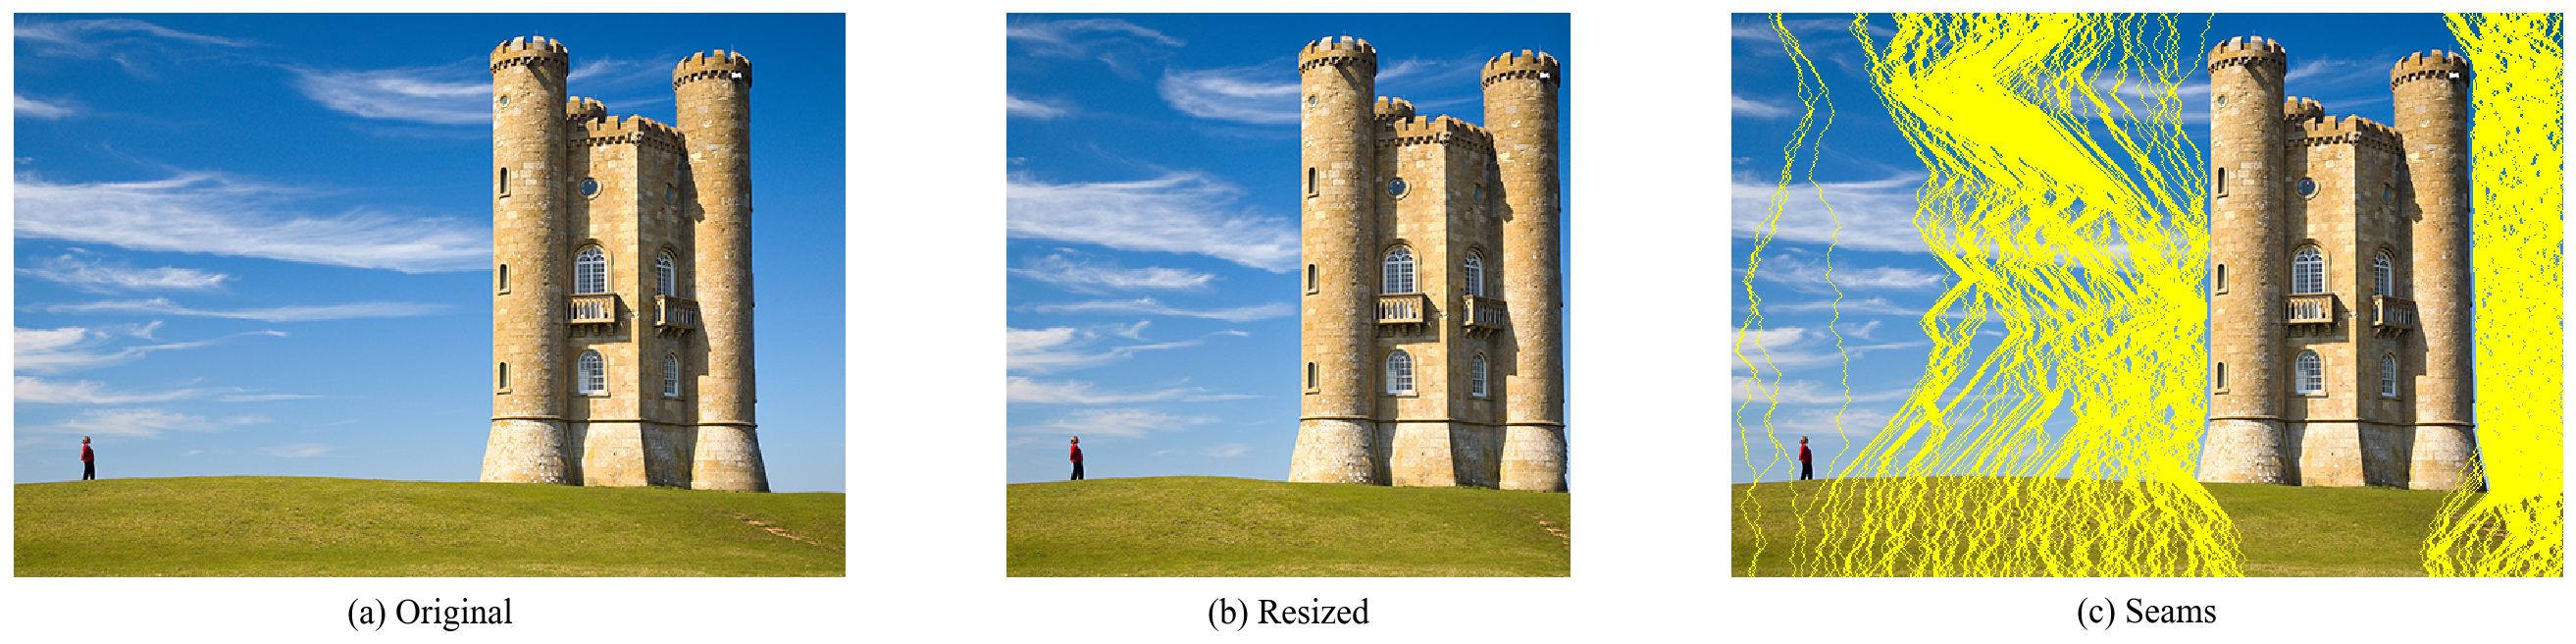
\includegraphics[width=\linewidth]{demo/output/castle.png}
    \vspace{-30pt}\caption{水平缩小}
    \label{fig:narrow_horiz}
\end{figure}\par
水平缩小如\Cref{fig:narrow_horiz},竖直缩小如\cref{fig:narrow_vert},均使用后向能量。可以看出细缝主要分布于诸如天空等梯度较小、重复区域较多的位置,其他梯度较大、信息较多的位置得以保留。
\begin{figure}[H]
    \centering
    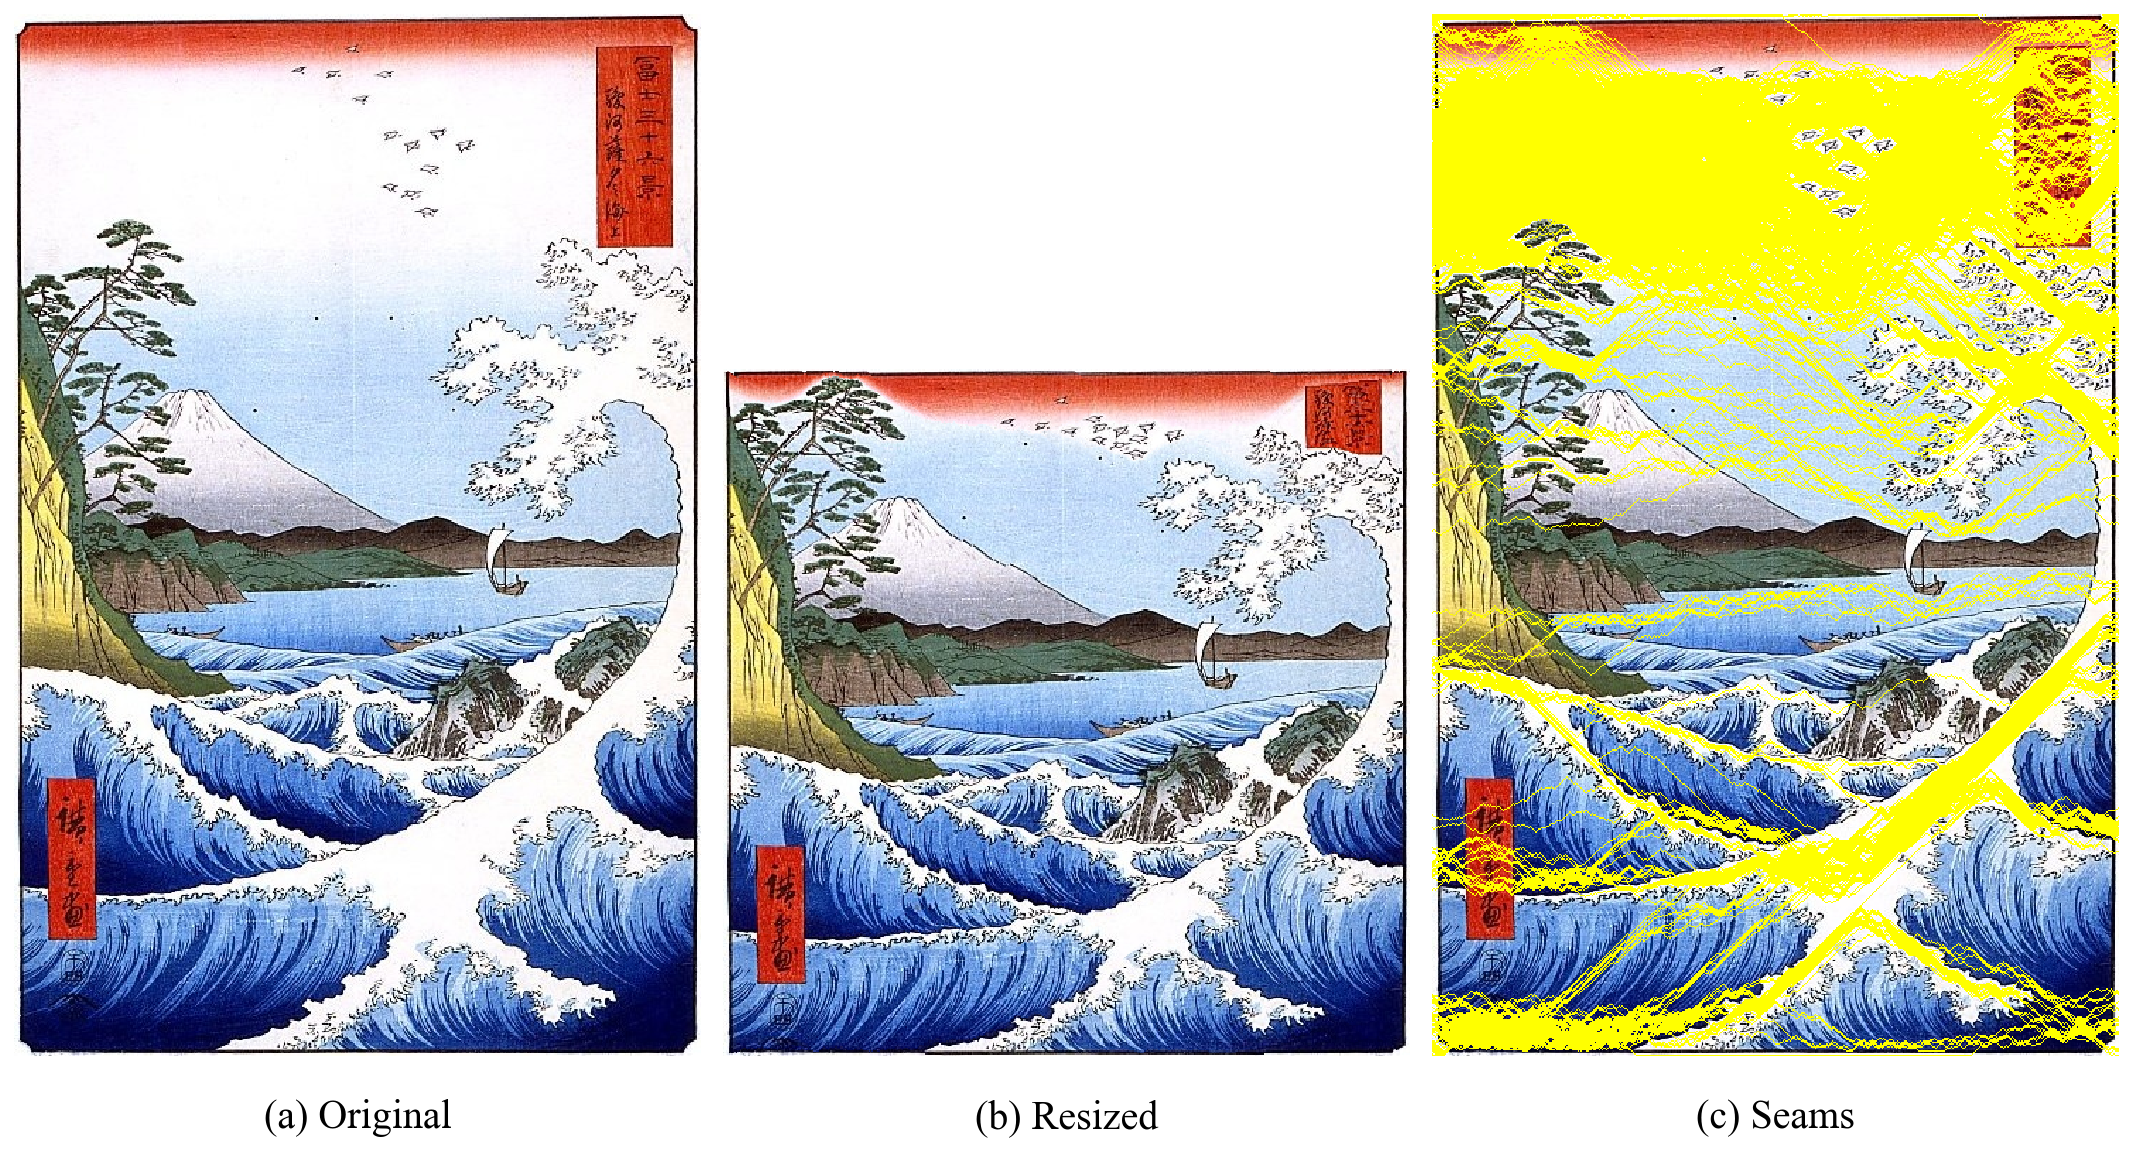
\includegraphics[width=\linewidth]{demo/output/fuji.png}
    \vspace{-30pt}\caption{竖直缩小}
    \label{fig:narrow_vert}
\end{figure}\par
上述方法存在局限性,如\cref{fig:narrow_fail_bw},使用后向能量时,主楼的形态被完全扭曲,边角的垂直关系被破坏;\cref{fig:narrow_fail_fw}使用前向能量时,主楼的边角垂直性得以保留,但整体形态呈现出类似于被压扁的效果。观察可知这个例子的图片明暗细节较为丰富,水平方向的冗余信息较少,而Seam Carving算法在这种情况下是难以得到较好效果的。
\begin{figure}[H]
    \centering
    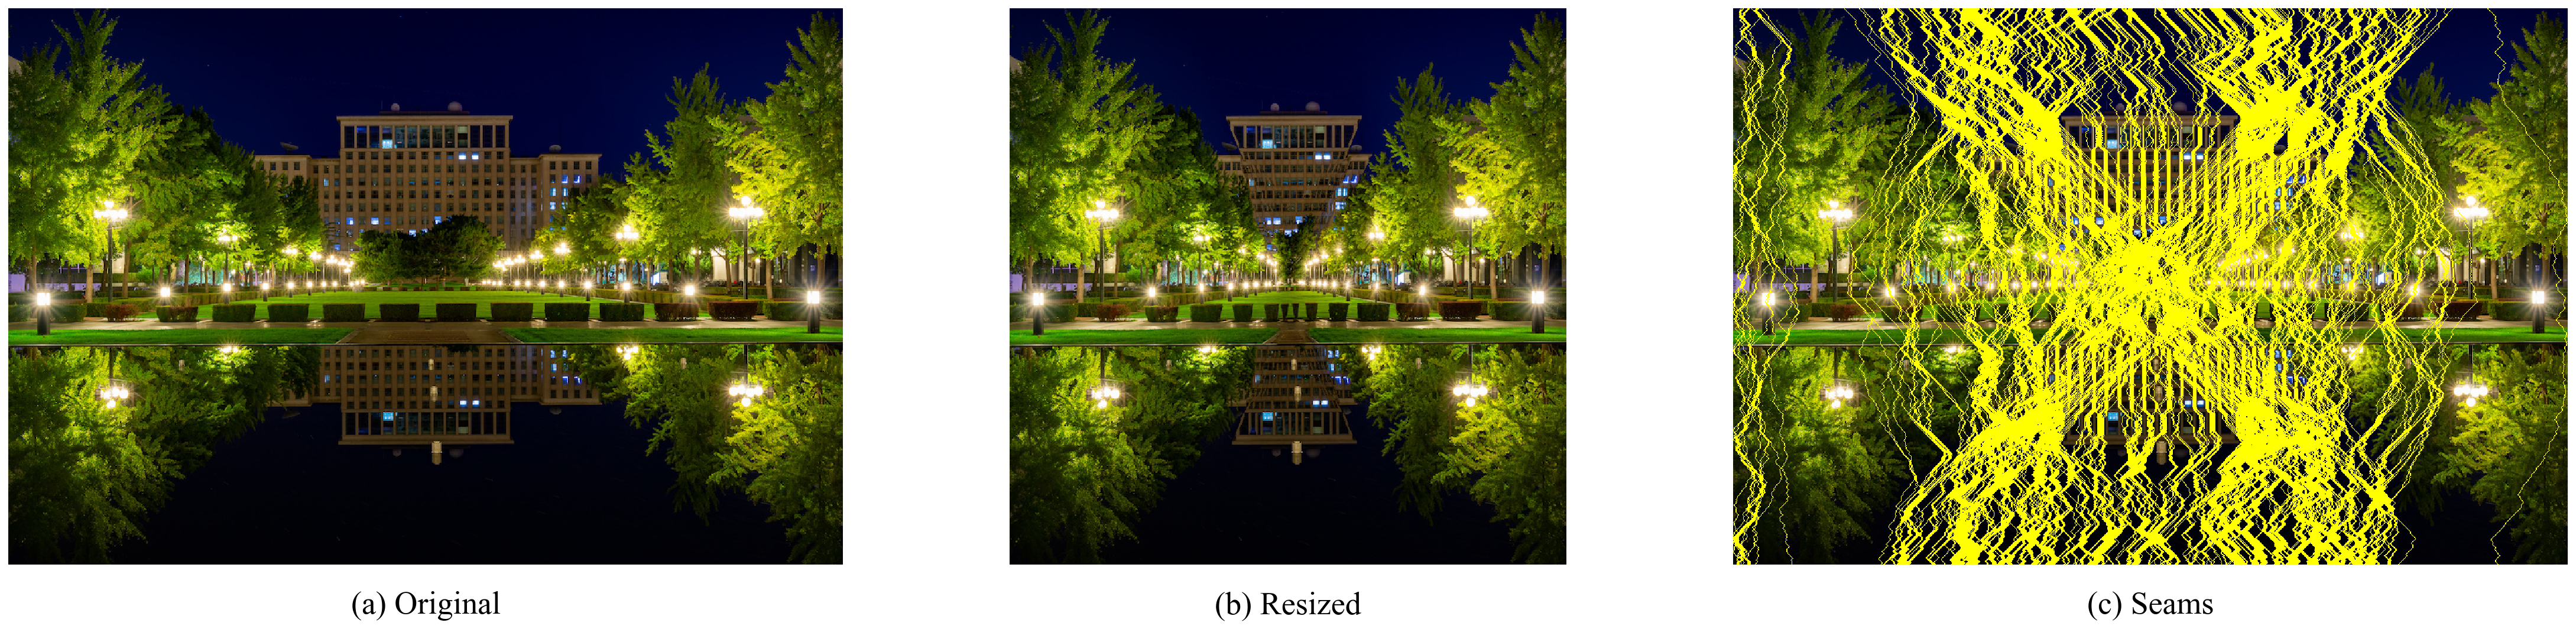
\includegraphics[width=\linewidth]{demo/output/mbuilding.png}
    \vspace{-30pt}\caption{水平缩小的失败例子(后向能量)}
    \label{fig:narrow_fail_bw}
\end{figure}\par
\begin{figure}[H]
    \centering
    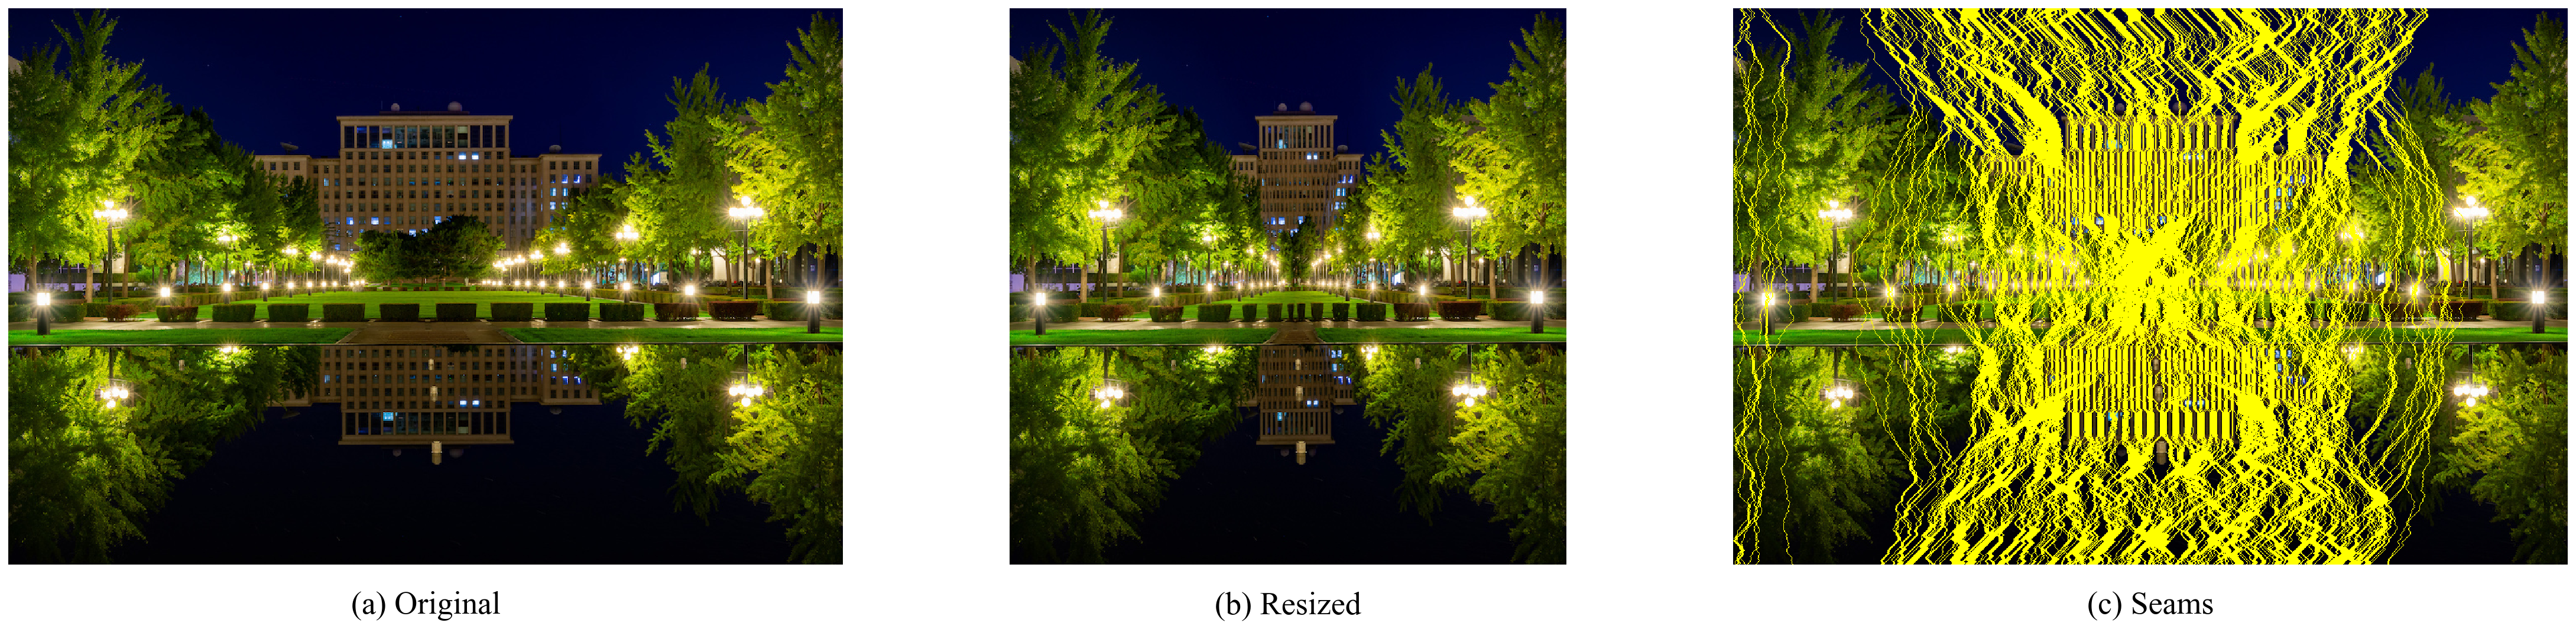
\includegraphics[width=\linewidth]{demo/output/mbuilding_forward.png}
    \vspace{-30pt}\caption{水平缩小的失败例子(前向能量)}
    \label{fig:narrow_fail_fw}
\end{figure}\par
\subsection{多种能量函数}
除了上面提到的仅使用$x,\,y$梯度信息$L$-1范数的$e_1$能量,这里还实现了基于Entropy的函数$e_{Entropy}$和HoG能量函数$e_{HoG}$(同时也附上前向能量与它们的对比,关于前向能量请参考扩展功能部分)。\par
$e_{Entropy}$的定义是在梯度能量$e_1$的基础上,增加图片的像素熵信息:
$$
 e_{Entropy}(x,y) = e_1(x,y) + Entropy(I(x, y)) = \left|\frac{\partial}{\partial x} I(i, j)\right| + \left|\frac{\partial}{\partial y} I(i, j)\right| + Entropy(I(x,y))
$$\par
这里使用$9\times9$的窗口来计算像素的熵信息。\par
$e_{HoG}$能量函数使用Histogram of Oriented Gradients (HoG)信息来对$e_1$进行归一化:
$$
 e_{HoG}(x, y) = \frac{e_1(x,y)}{\max{(HoG(I(x,y)))}}
$$\par
HoG的思想是将梯度的方向(角度,范围为$[0,\,2\pi]$)划分为多个bin,使用在bin内出现的梯度的幅值(可以是梯度的$L$-2范数)来统计频率。这里HoG的计算使用$11\times 11$窗口,取$8$个方向的bin。\par
这里使用\cite{avidan2007seam}中的样例,原图如下
\begin{figure}[H]
    \centering
    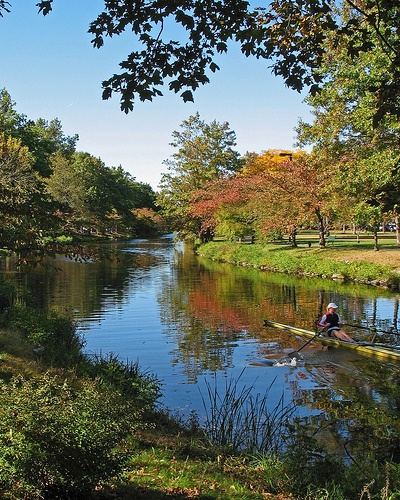
\includegraphics[width=0.4\linewidth]{demo/orig/charles.jpg}
    \caption{样例Charles原始图像}
    \label{fig:multi_energy_func_orig}
\end{figure}\par

结果如\Cref{fig:charles_e1,,fig:charles_ent,,fig:charles_hog,,fig:charles_efw}所示,这里展示了能量函数、累积能量(竖直方向)以及原图缩小后的结果。
\begin{figure}[H]
    \centering
    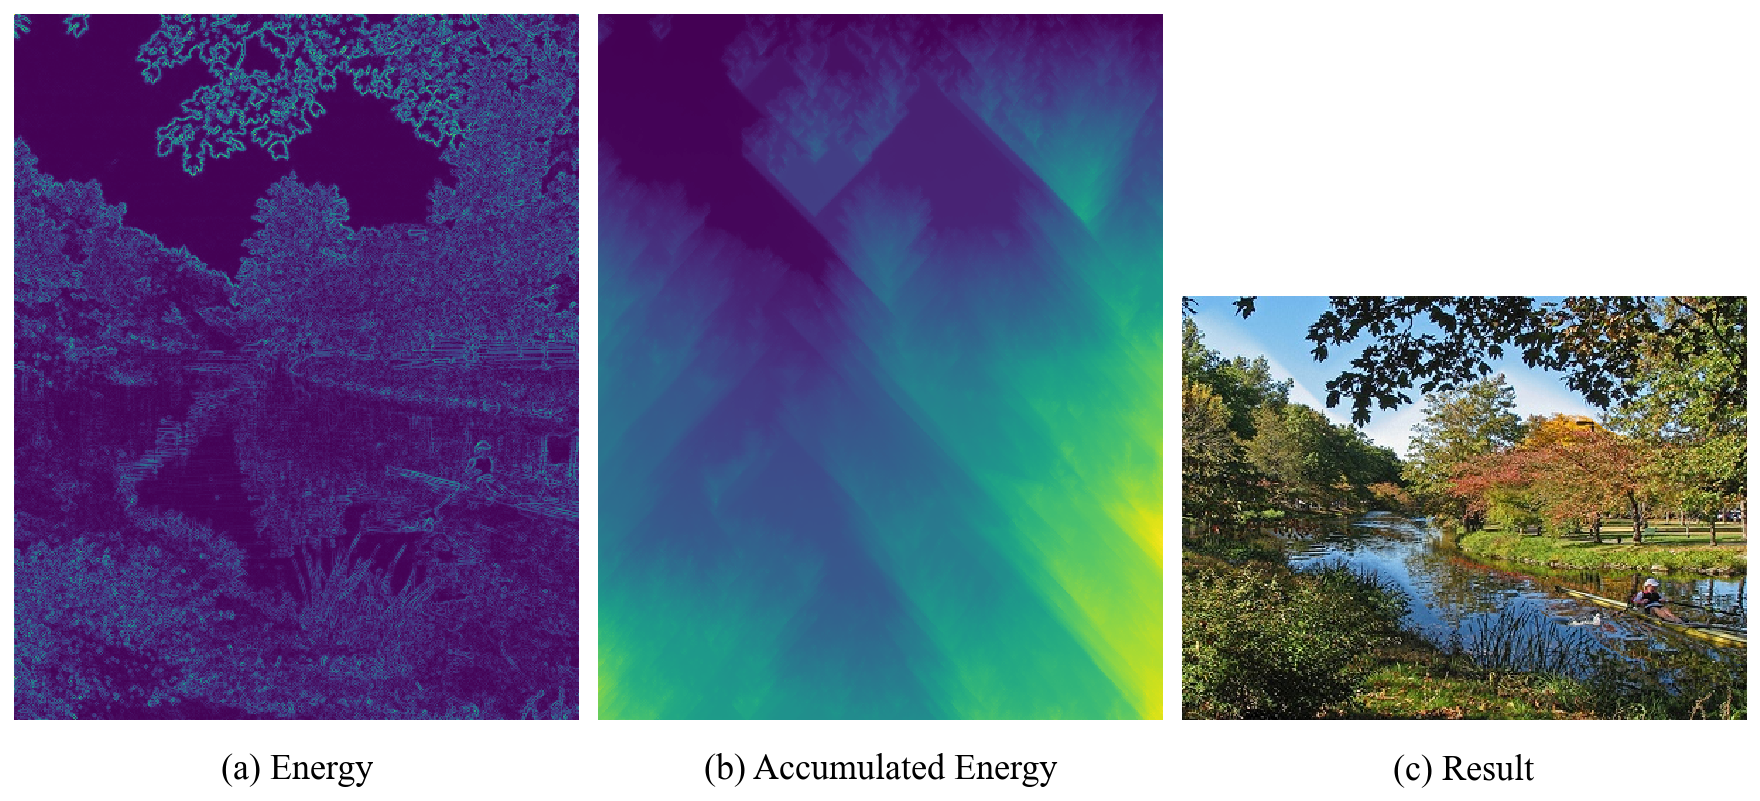
\includegraphics[width=\linewidth]{demo/output/charles_gradient.png}
    \vspace{-30pt}\caption{$e_1$能量函数}
    \label{fig:charles_e1}
\end{figure}\par

\begin{figure}[H]
    \centering
    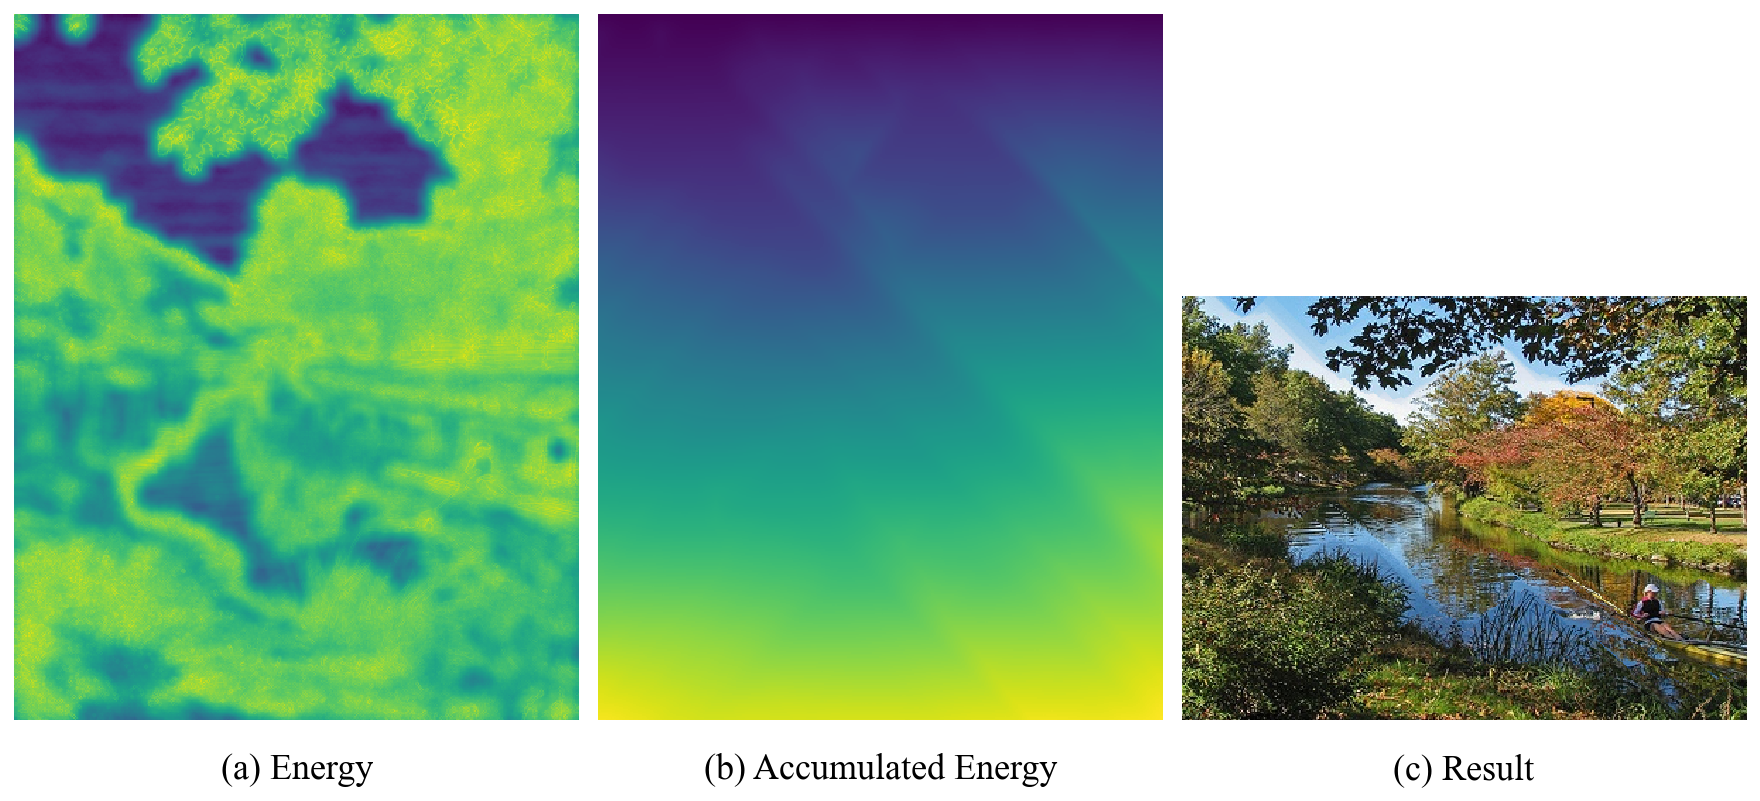
\includegraphics[width=\linewidth]{demo/output/charles_entropy.png}
    \vspace{-30pt}\caption{$e_{Entropy}$能量函数}
    \label{fig:charles_ent}
\end{figure}\par

\begin{figure}[H]
    \centering
    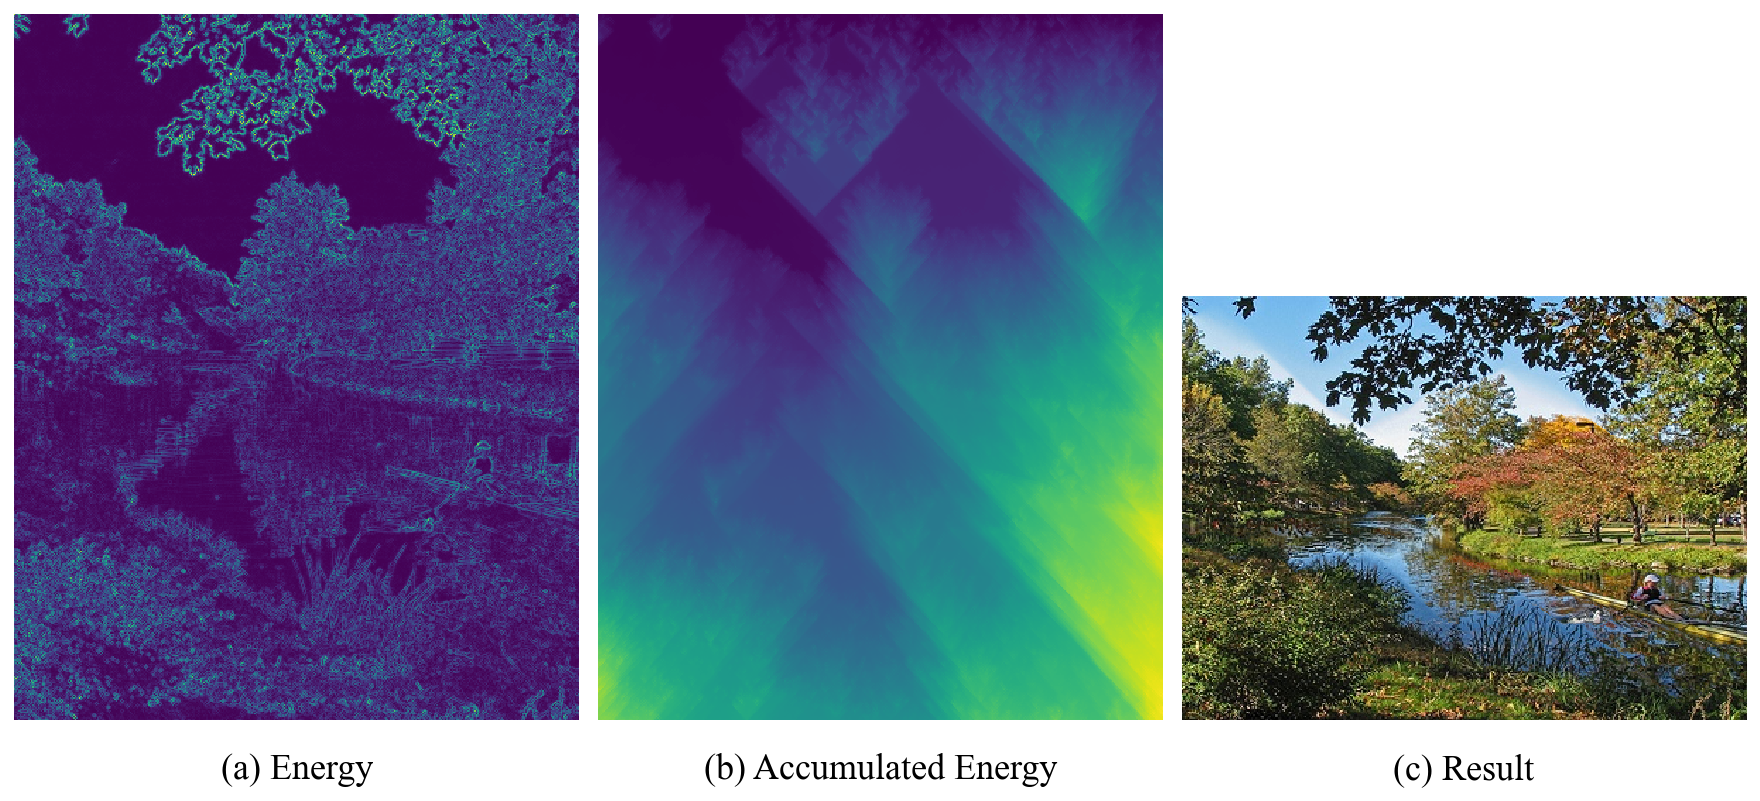
\includegraphics[width=\linewidth]{demo/output/charles_hog.png}
    \vspace{-30pt}\caption{$e_{HoG}$能量函数}
    \label{fig:charles_hog}
\end{figure}\par

\begin{figure}[H]
    \centering
    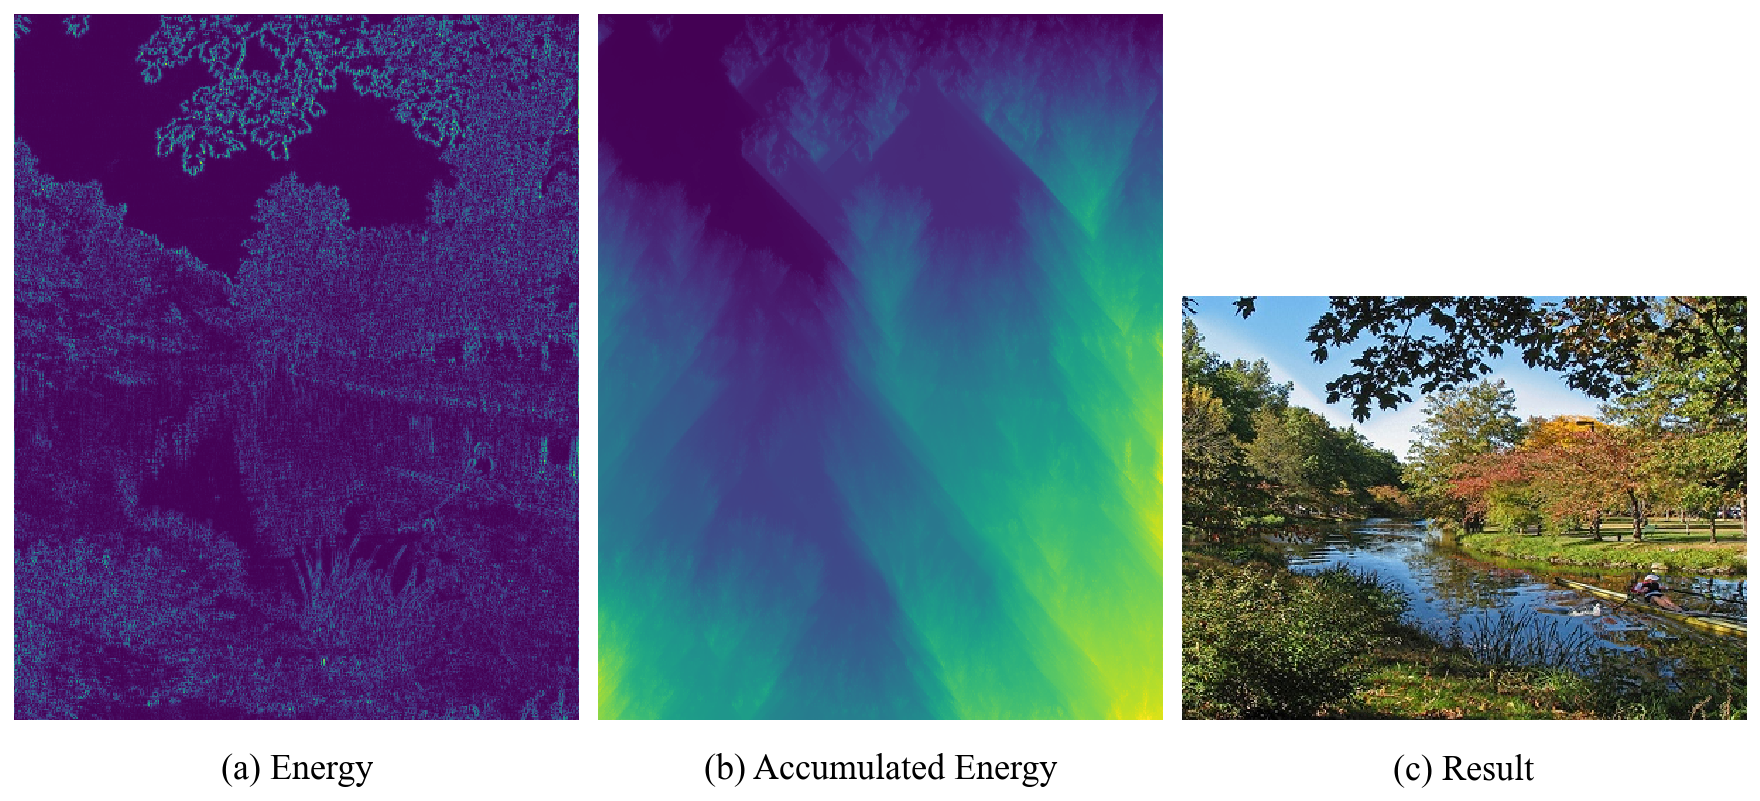
\includegraphics[width=\linewidth]{demo/output/charles_forward.png}
    \vspace{-30pt}\caption{前向能量函数}
    \label{fig:charles_efw}
\end{figure}
\section{扩展功能}
\subsection{图像扩展}
在上述Seam Carving图像缩小的算法基础上,可以推广为图像扩展算法。具体操作是将选取的细缝扩充一份,它的颜色值取原细缝左右两边像素的平均值。如果选取了$n$条这样的细缝,可以将图片的宽或高增加$n$个像素。根据扩展的顺序,可以有三种处理方法:
\begin{itemize}
    \item 迭代扩展:每次只扩展一条细缝,重复$n$次;
    \item 统一扩展:算出$n$条细缝后统一扩展;
    \item 分阶段扩展:限制统一扩展每次增加的细缝数,分为多个阶段进行扩展。
\end{itemize}
这些方法的效果如\cref{fig:expansion_methods}所示:
\begin{figure}[H]
    \centering
    \subfigure[原图]{
        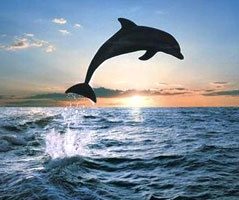
\includegraphics[height=4.5cm]{demo/orig/dolphin.jpg}
    }
    \subfigure[迭代扩展]{
        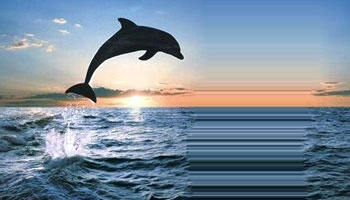
\includegraphics[height=4.5cm]{demo/output/dolphin_exapnd_single.jpg}
    }
    \\
    \subfigure[统一扩展]{
        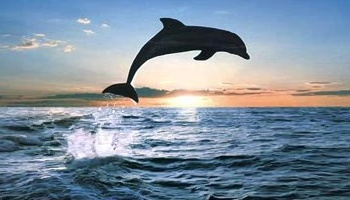
\includegraphics[height=4.5cm]{demo/output/dolphin_exapnd_multi.jpg}
    }
    \\
    \subfigure[分阶段扩展(阶段1)]{
        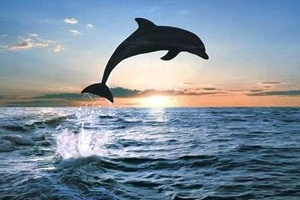
\includegraphics[height=4.5cm]{demo/output/dolphin_exapnd_multi_phase_1.jpg}
    }
    \subfigure[分阶段扩展(阶段2)]{
        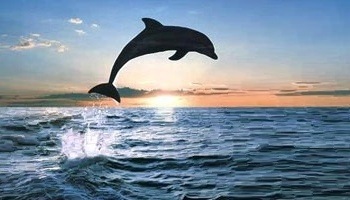
\includegraphics[height=4.5cm]{demo/output/dolphin_exapnd_multi_phase_2.jpg}
    }
    \caption{多种扩展方法的效果对比}
    \label{fig:expansion_methods}
\end{figure}\par
可以看出,迭代扩展容易每次选择相同的细缝进行扩展,出现了图中的像素重复现象;统一扩展解决了这样的问题,但容易使得图中物体发生明显形变(图中海豚被拉宽了);分阶段扩展限制每次扩展的宽度,最后得到的结果相比统一扩展更好。
\subsection{目标保护/移除}
通过对能量函数引入额外信息,可以实现目标的保护或移除。对于需要保护的像素,将它们的能量加上一个较大常数$P$;对于需要移除的像素,将能量减去较大值$R$即可。实际实现时,需要满足$R \gg P$,否则在保护和移除共存的情况下,将难以得到可行的细缝。另外注意这里是给mask内的像素的能量加上常数偏置,而不是直接将能量设置为常数,这样可以保留原有像素的梯度能量等信息。\par
在图像缩小较多时,图像中主体可能发生较大形变,需要进行保护,如\Cref{fig:ratatouille}所示:
\begin{figure}[H]
    \centering
    \subfigure[原图]{
        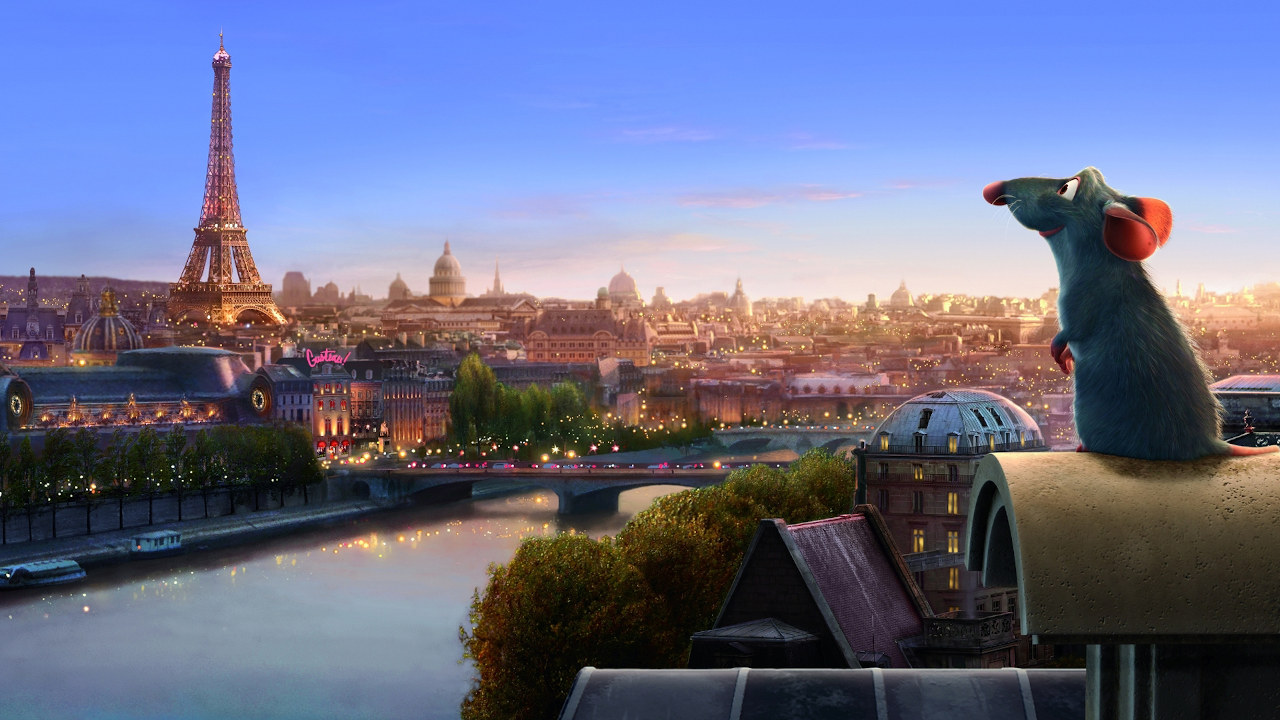
\includegraphics[height=4.5cm]{demo/orig/ratatouille.jpg}
    }
    \\
    \subfigure[缩小宽度]{
        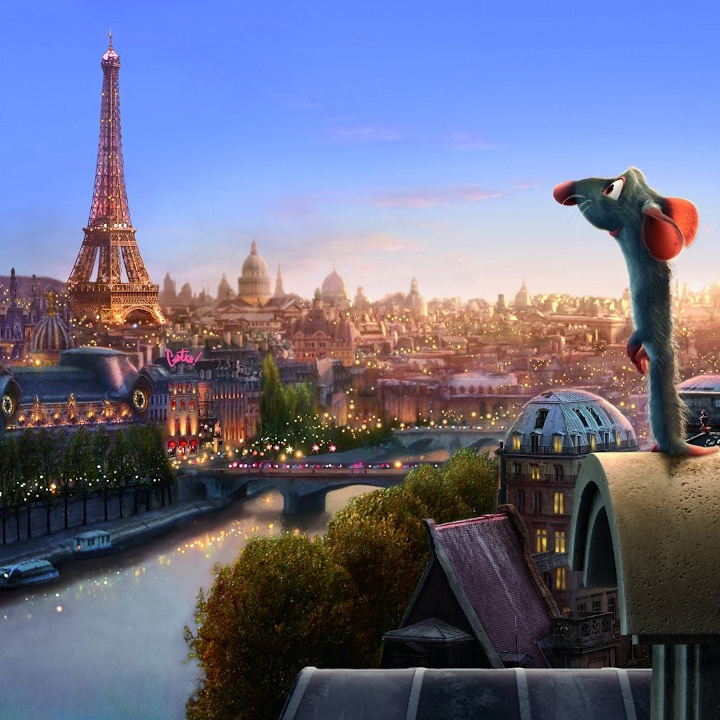
\includegraphics[height=6cm]{demo/output/ratatouille_fail.jpg}
    }
    \subfigure[保护主体对象]{
        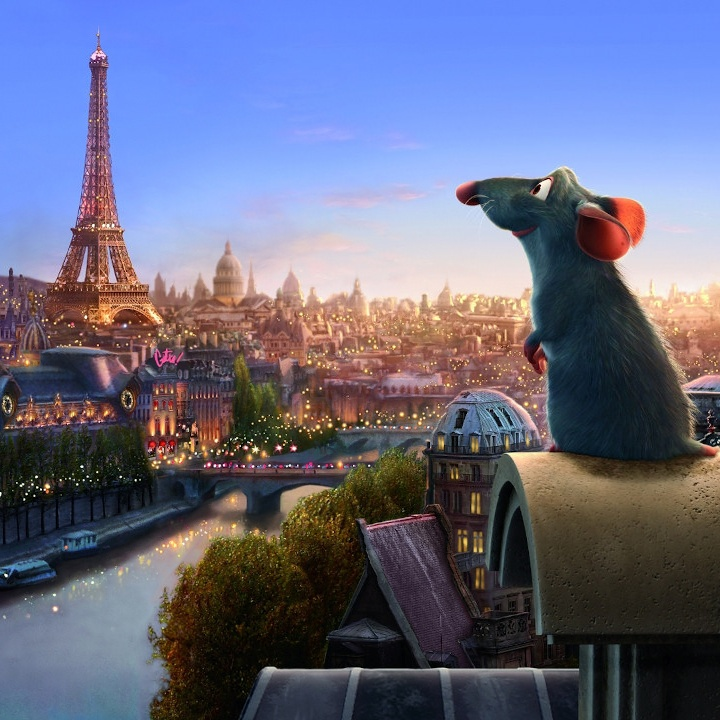
\includegraphics[height=6cm]{demo/output/ratatouille_success.jpg}
    }
    \caption{目标保护示例}
    \label{fig:ratatouille}
\end{figure}\par
目标移除效果如图\Cref{fig:shoes_removal},这里同时使用了移除对象和保护对象的mask(移除第一行的左四粉色鞋,同时保护它两侧的鞋):
\begin{figure}[H]
    \centering
    \subfigure[原图]{
        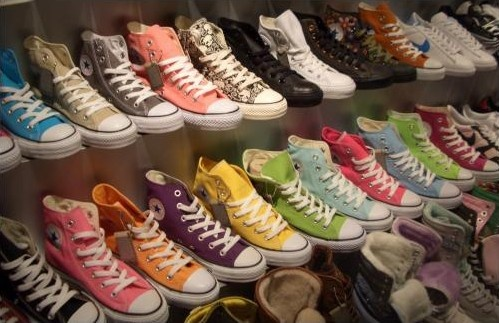
\includegraphics[height=3cm]{demo/orig/shoes.jpg}
    }
    \subfigure[移除目标]{
        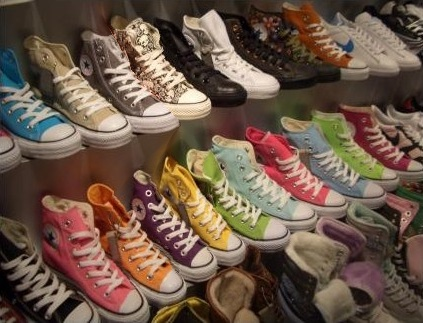
\includegraphics[height=3cm]{demo/output/shoes_removed.jpg}
    }
    \subfigure[扩充到原宽度]{
        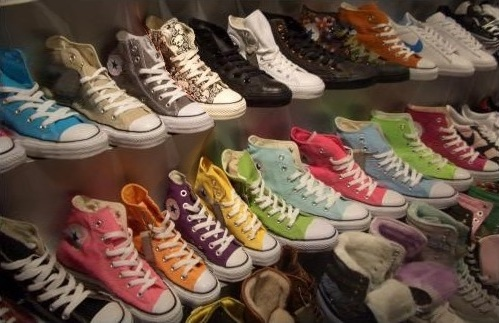
\includegraphics[height=3cm]{demo/output/shoes_final.jpg}
    }
    \caption{目标移除示例}
    \label{fig:shoes_removal}
\end{figure}\par
\subsection{改进的能量公式}
\subsubsection{前向能量}
传统的Seam Carving使用后向能量,它只考虑移除细缝前的像素梯度信息。\cite{rubinstein2008improved}对此进行改进,提出了前向能量,思想如下:
\begin{figure}[H]
    \centering
    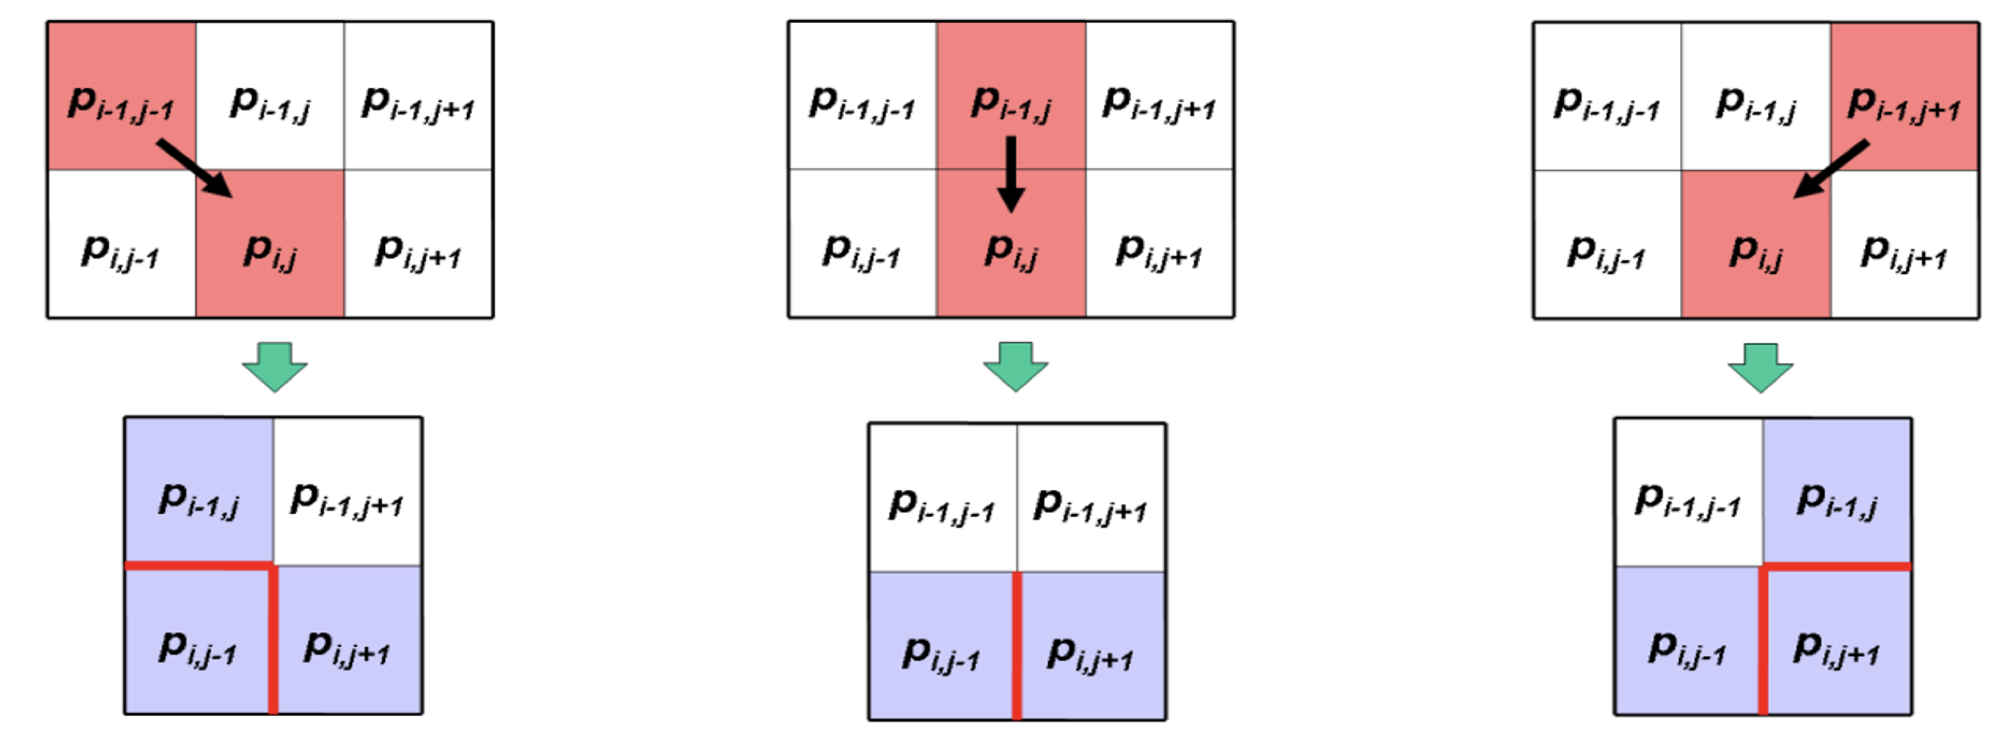
\includegraphics[width=0.8\linewidth]{demo/fw_energy.png}
    \caption{前向能量的原理}
    \label{fig:fw_energy_inner}
\end{figure}\par
前向能量主要考虑的是细缝移除后的产生的图像不连续性。如上图的像素$(i,j)$,如果细缝穿过它,会使得原来不相邻的$(i,j-1),\,(i,j+1)$像素相邻(产生了一个新的不连续点),而根据细缝在前一行的位置,又有可能产生新的不连续点:
\begin{itemize}
    \item 细缝经过$(i-1,j-1)$,移除细缝后,$(i-1,j),(i,j-1)$相邻,产生新的不连续;
    \item 细缝经过$(i-1,j)$,移除细缝后,除了前一行的不连续外,没有产生新的不连续;
    \item 细缝经过$(i,j+1)$,$(i-1,j),(i,j+1)$产生新的不连续
\end{itemize}\par
这些不连续在上图中使用红色标出。定义每个像素的能量为选取细缝情况的不连续程度,使用不连续点处的梯度的绝对值表示:
\begin{equation}
    \begin{split}
        C_L(i,j) &= |I(i,j+1)-I(i,j-1)| + |I(i-1,j)-I(i,j-1)|\\
        C_U(i,j) &= |I(i,j+1)-I(i,j-1)| \\
        C_R(i,j) &= |I(i,j+1)-I(i,j-1)| + |I(i-1,j)-I(i,j+1)|
    \end{split}
\end{equation}\par
类似于计算细缝的过程,这个能量也可以用动态规划求得:
\begin{equation}
    M(i,j) = 
    \begin{cases}
        M(i-1,j-1) + C_L(i,j) \\
        M(i-1,j) + C_U(i,j) \\
        M(i-1,j+1) + C_R(i,j)
    \end{cases}
\end{equation}\par
这里使用\cite{rubinstein2008improved}中的例子,结果如\Cref{fig:bw_energy,,fig:fw_energy}所示
\begin{figure}[H]
    \centering
    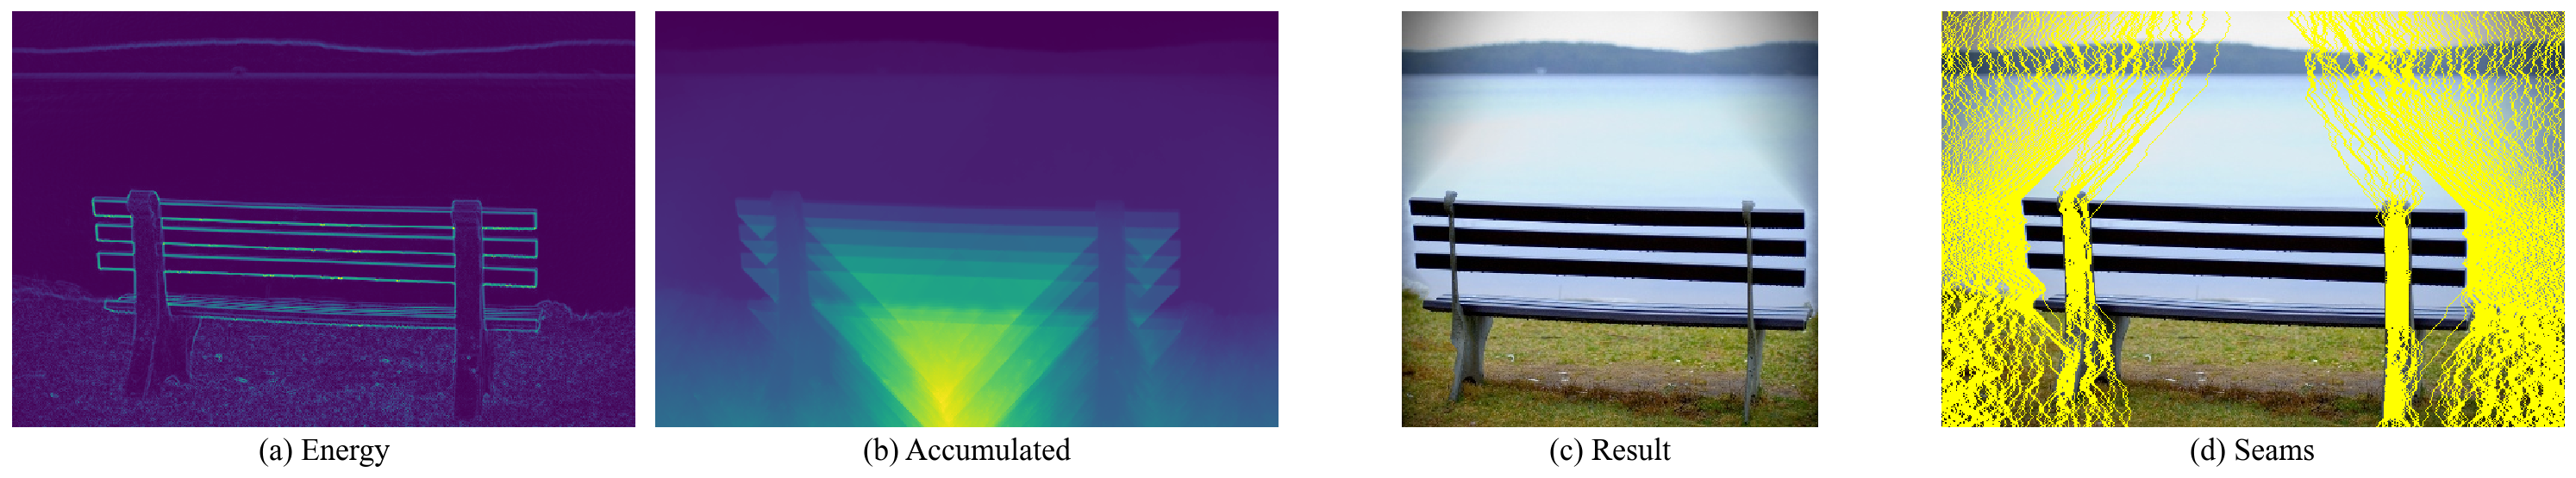
\includegraphics[width=\linewidth]{demo/output/backward_energy.png}
    \vspace{-30pt}\caption{后向能量}
    \label{fig:bw_energy}
\end{figure}\par
\begin{figure}[H]
    \centering
    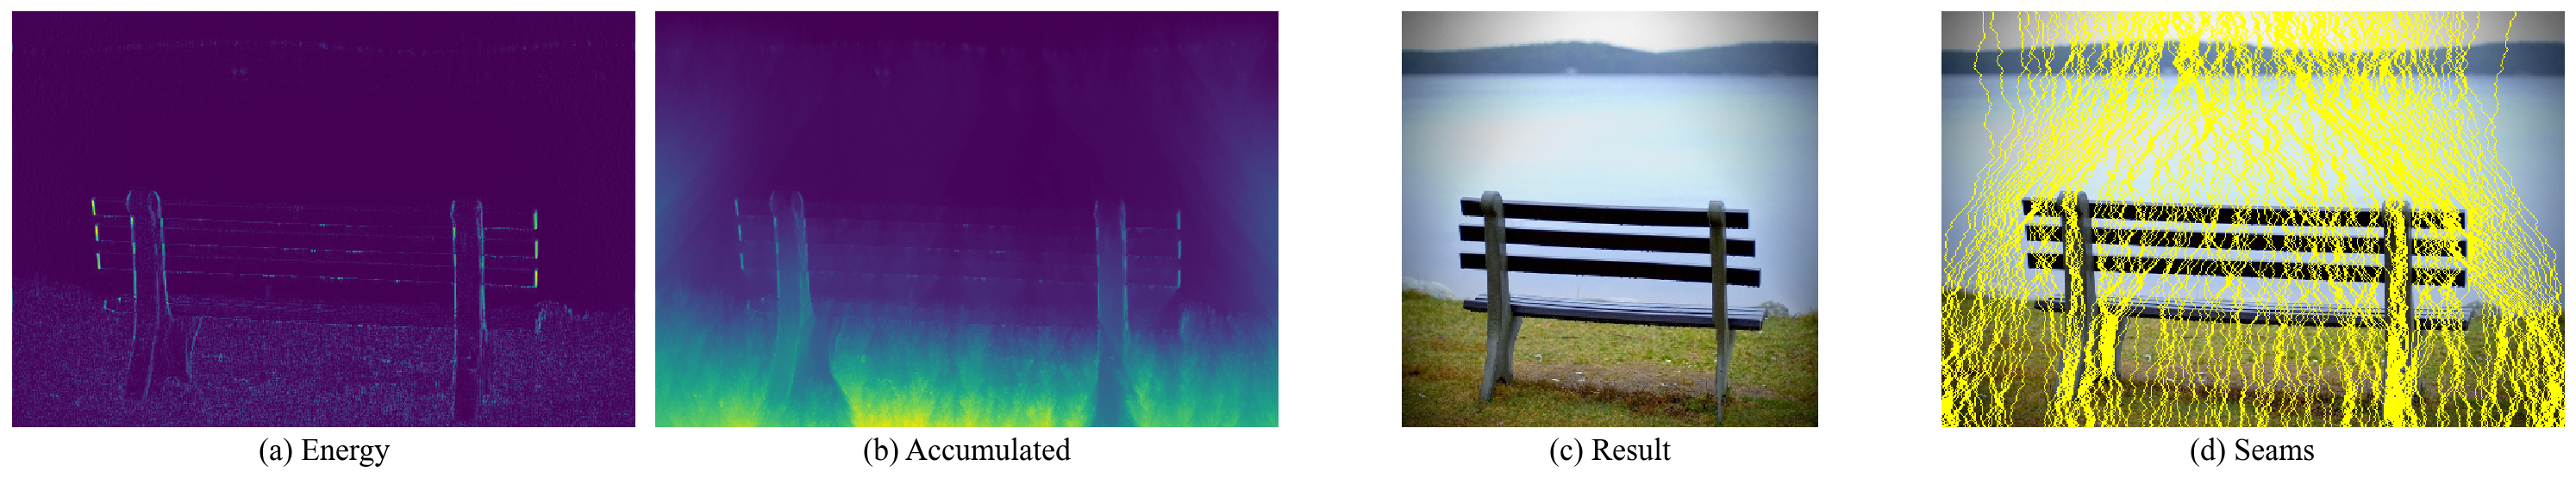
\includegraphics[width=\linewidth]{demo/output/forward_energy.png}
    \vspace{-30pt}\caption{前向能量}
    \label{fig:fw_energy}
\end{figure}
\subsubsection{处理人脸}
在背景颜色较为丰富的图片中做缩小,容易对人脸等结构性较强的物体造成扭曲,如\Cref{fig:face_prot}
\begin{figure}[H]
    \centering
    \subfigure[原图]{
        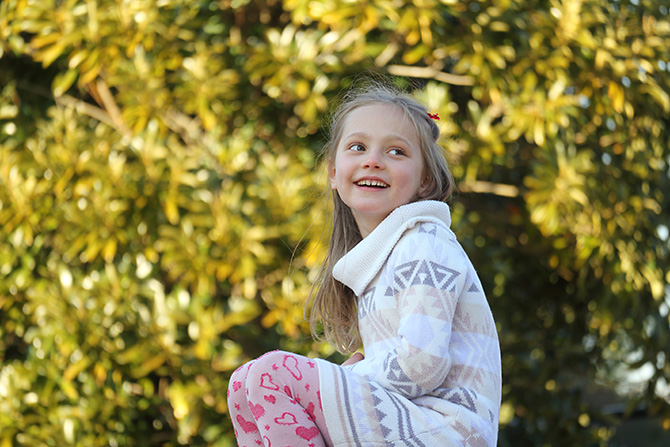
\includegraphics[height=4cm]{demo/orig/face.jpg}
    }
    \subfigure[不保护人脸的结果]{
        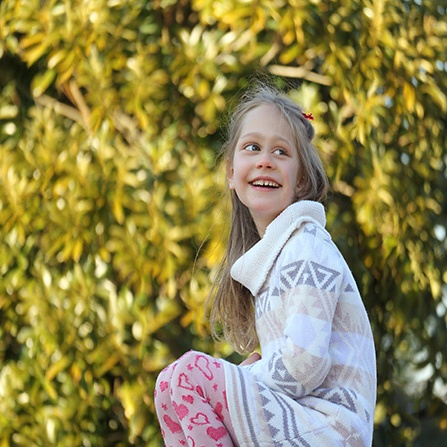
\includegraphics[height=4cm]{demo/output/face_fail.jpg}
    }
    \subfigure[保护人脸]{
        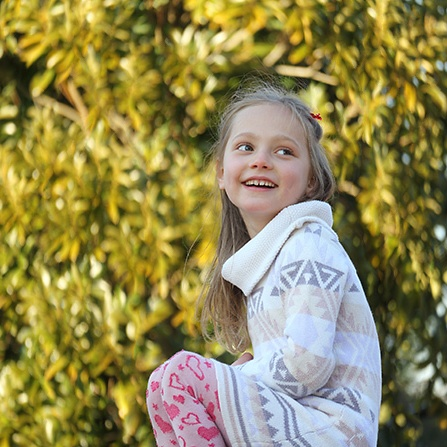
\includegraphics[height=4cm]{demo/output/face_success.jpg}
    }
    \caption{不同方式处理含人脸图片的结果}
    \label{fig:face_prot}
\end{figure}\par
这里使用基于\texttt{dlib}的人脸检测器,得到人脸的包围框后,将其加入目标保护的mask中。从结果中可以看出,这种方法得到的人脸结构被完整保留下来了。
\subsection{优化的删缝顺序}
如果需要同时对图片的宽高进行调整,先宽后高或者先高后宽的策略并不一定是最优的。定义调整的总能量为调整过程中所有细缝的能量和,则最优的方法是最小化该能量
$$
\min_{s^x,s^y,\alpha} \sum_{i=1}^n E(\alpha_i s^x_i + (1-\alpha_i)s^y_i)
$$\par
上式中$s^x,s^y$分别为水平和竖直细缝,$\alpha$为表示细缝方向的序列,$\alpha=1$表示水平细缝。显然上述最小总能量可以使用动态规划求解。记$\mathbf{T}(r,c)$为将原图缩小$r$行$c$列的最小能量,那么有
$$
\mathbf{T}(r,c) = \min \left\{ \mathbf{T}(r-1,c) + E(s^x (I_{(n-(r-1)) \times (m-c)}) ), \mathbf{T}(r,c-1) + E(s^y(I_{(n-r) \times (m-(c-1))} ) ) \right\}
$$\par
\begin{figure}[H]
    \centering
    \subfigure[原图]{
        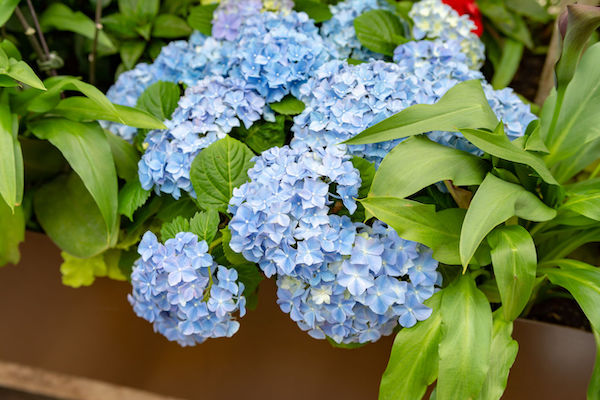
\includegraphics[height=4cm]{demo/orig/flower.jpg}
    }
    \subfigure[$T$矩阵以及最优路径]{
        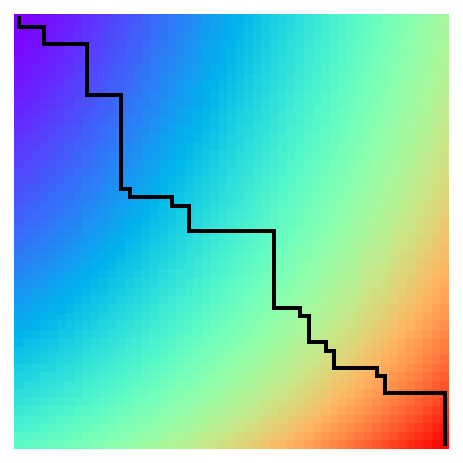
\includegraphics[height=4cm]{demo/output/optim_order_seam.png}
    }
    \subfigure[最优缩小结果]{
        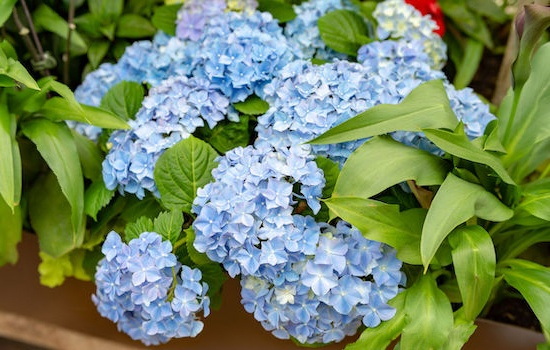
\includegraphics[height=3.5cm]{demo/output/optim_order_out.jpg}
    }
    \caption{最优删缝顺序(长宽均减小50像素)}
    \label{fig:optim_order}
\end{figure}\par
\subsection{Gradient Domain Carving with Poisson Solver}
在删除细缝后,原图中不相邻的像素将直接相邻,它们的颜色差值可能较大。为了使得它们的过渡更加自然,根据\cite{avidan2007seam},可以使用\cite{Perez03a}的Poisson Image Editing算法。主要步骤是在计算原图的Laplacian后,移除梯度域的细缝,再使用Poisson Solver重建图像。\par
注意移除梯度图的细缝后,需要维护Dirichlet边界条件,记梯度图为$\mathcal{L}$,如果有一条竖直细缝穿过像素$(i,j)$,会使得$(i,j-1)$和$(i,j+1)$直接相邻,它们成为新的边界,那么需要
$$
\begin{aligned}
    \mathcal{L}'(i,j-1) & = \mathcal{L}(i,j-1) + I(i, j-1) \\
    \mathcal{L}'(i,j+1) & = \mathcal{L}(i,j-1) + I(i, j-1) \\
\end{aligned}
$$\par
这里统一使用细缝左侧边界的颜色信息作为边界条件,以保持细缝两侧的一致性。对于水平细缝,统一使用上侧的颜色作为边界。如果细缝使得原来图像的内点变为整个图片的边界,则取原图中该像素的颜色作为边界即可。\par
下图是使用Poisson Solver进行目标移除的效果,可以看出边缘相比直接移除明显更加平滑。
\begin{figure}[H]
    \centering
    \subfigure[原图]{
        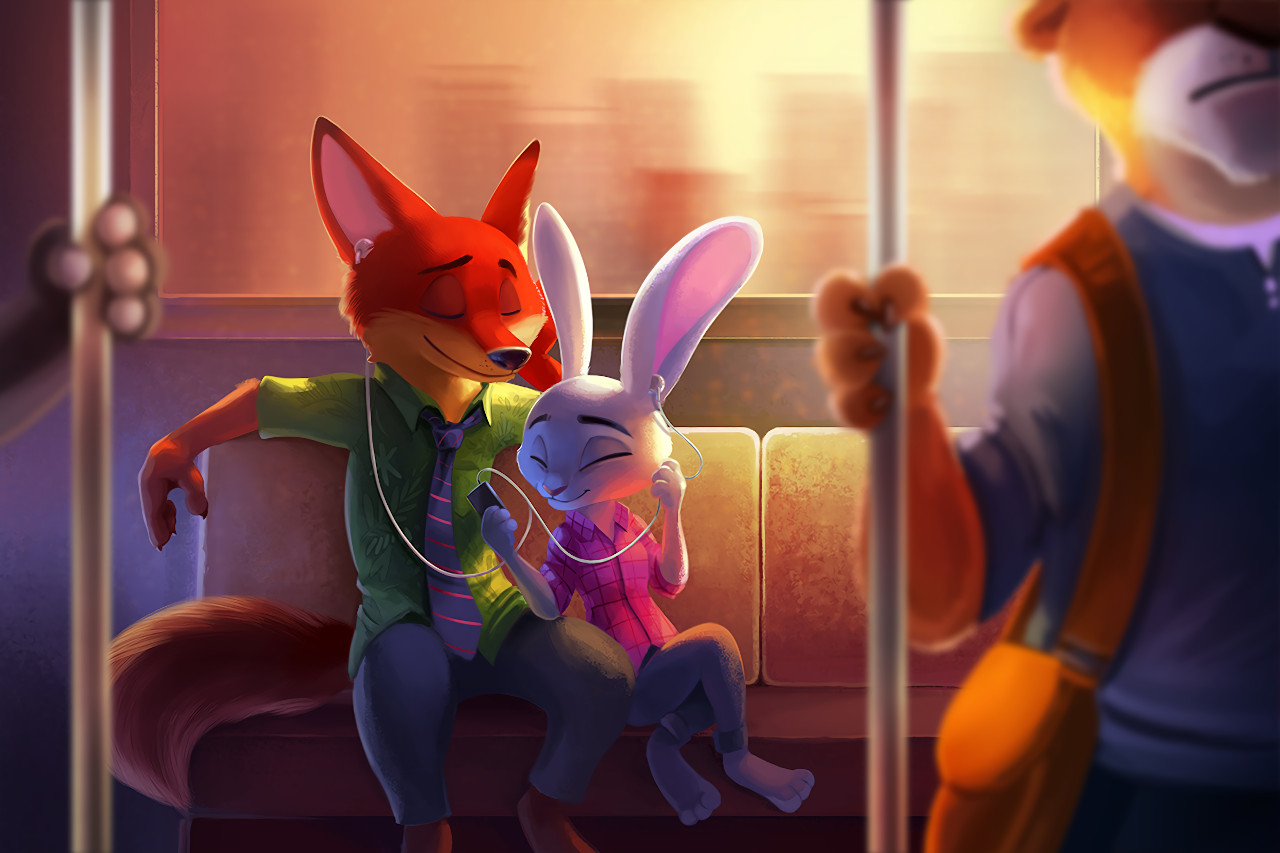
\includegraphics[height=4cm]{demo/orig/zootopia.jpg}
    }
    \subfigure[直接目标移除]{
        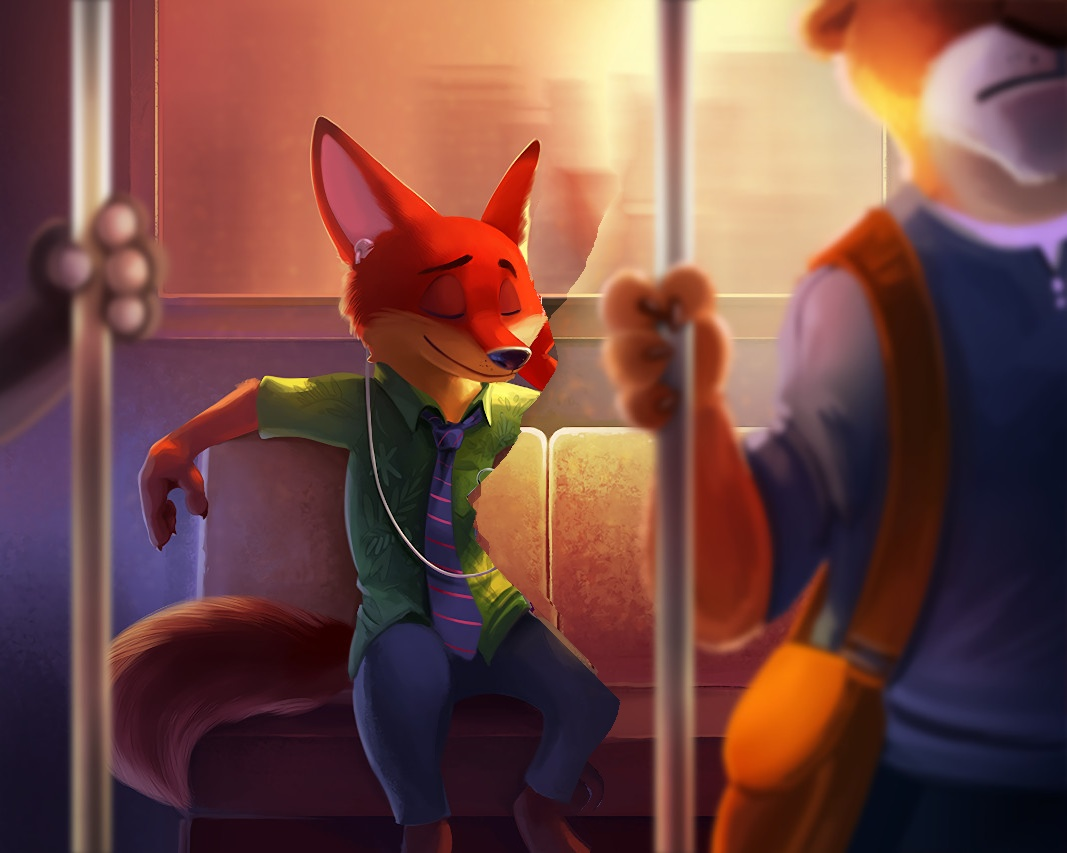
\includegraphics[height=4cm]{demo/output/zootopia_plain.jpg}
    }
    \\
    \subfigure[使用Poisson Solver的目标移除]{
        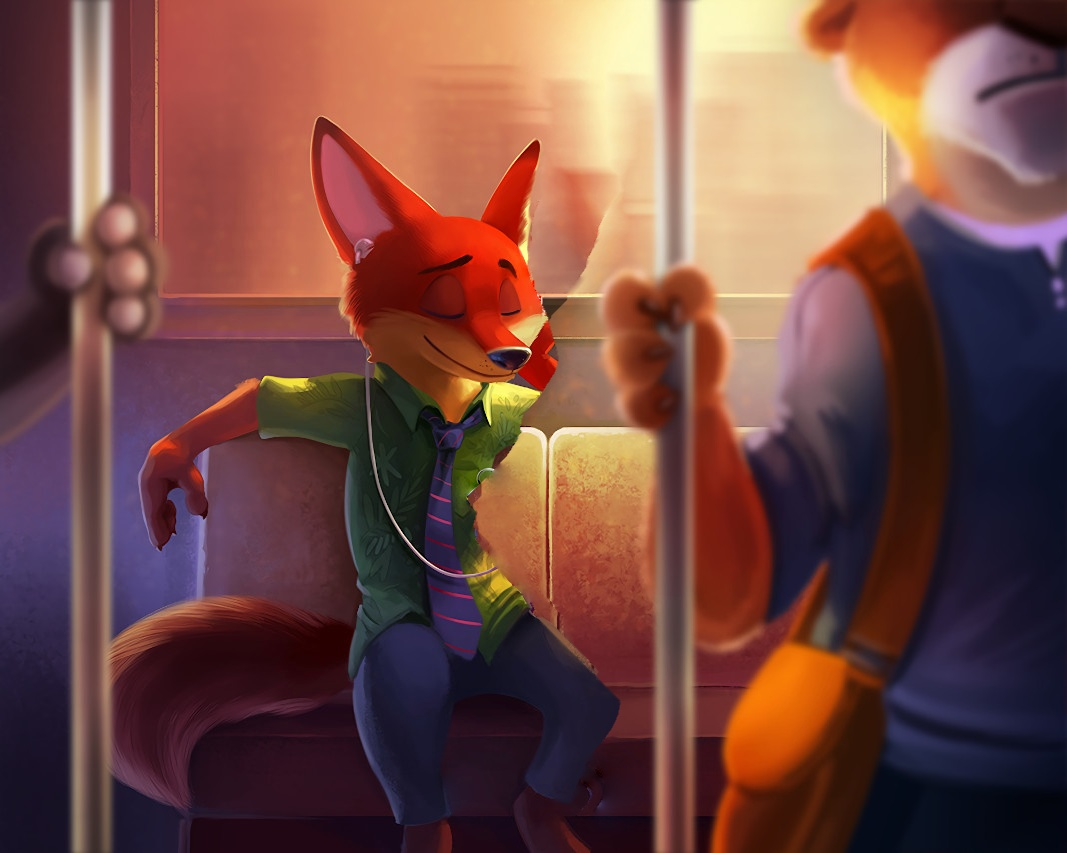
\includegraphics[height=4cm]{demo/output/zootopia_poisson.jpg}
    }
    \subfigure[图片扩展为原宽度]{
        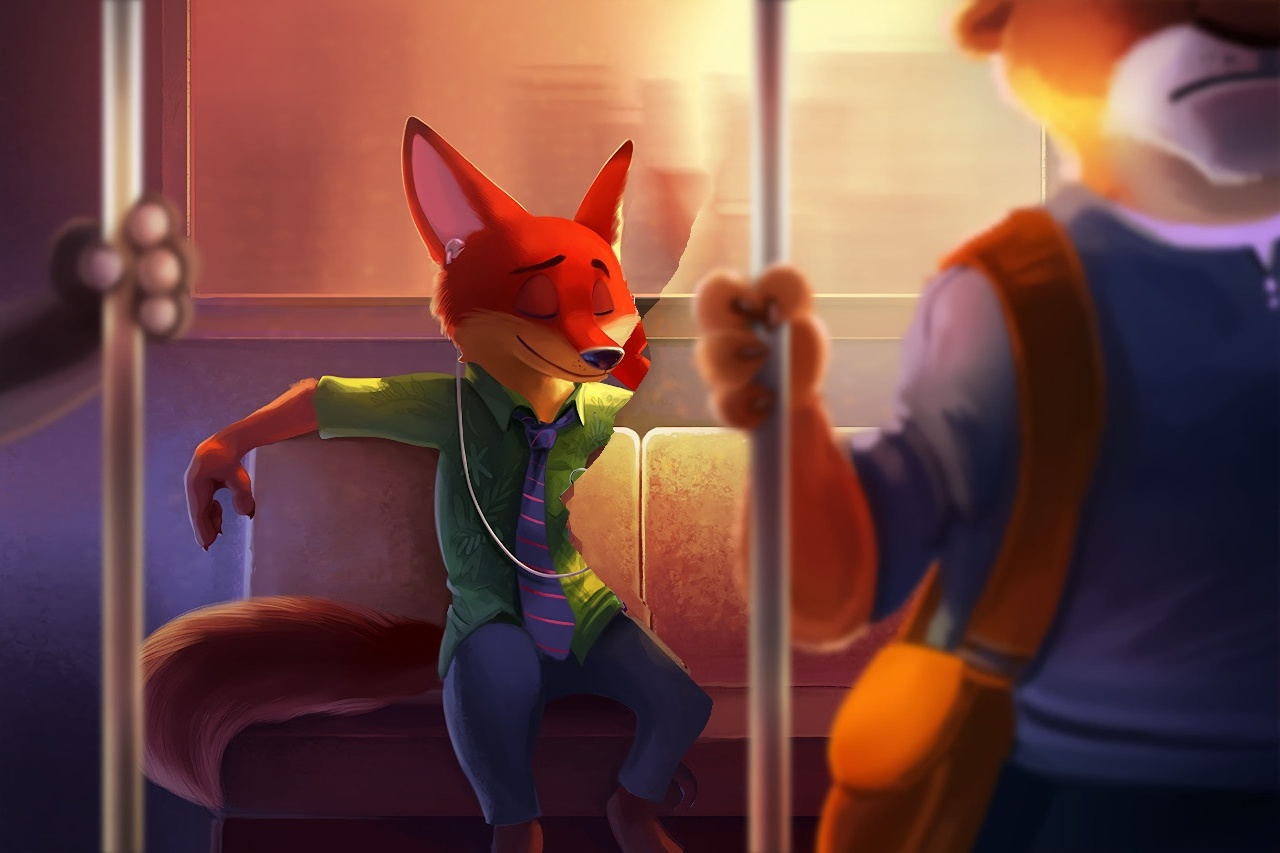
\includegraphics[height=4cm]{demo/output/zootopia_remove_expanded.jpg}
    }
    \\
    \subfigure[直接目标移除(局部)]{
        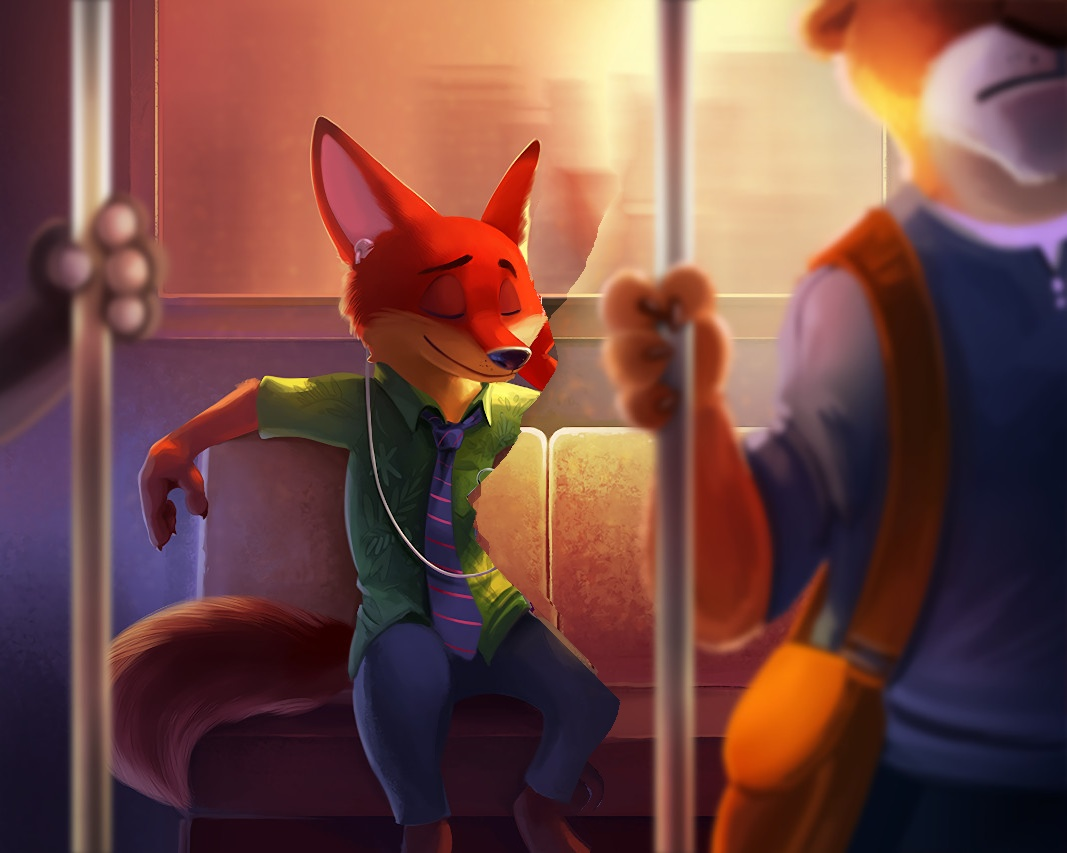
\includegraphics[height=4cm,trim=350 200 350 400,clip]{demo/output/zootopia_plain.jpg}
    }
    \subfigure[使用Poisson Solver的目标移除(局部)]{
        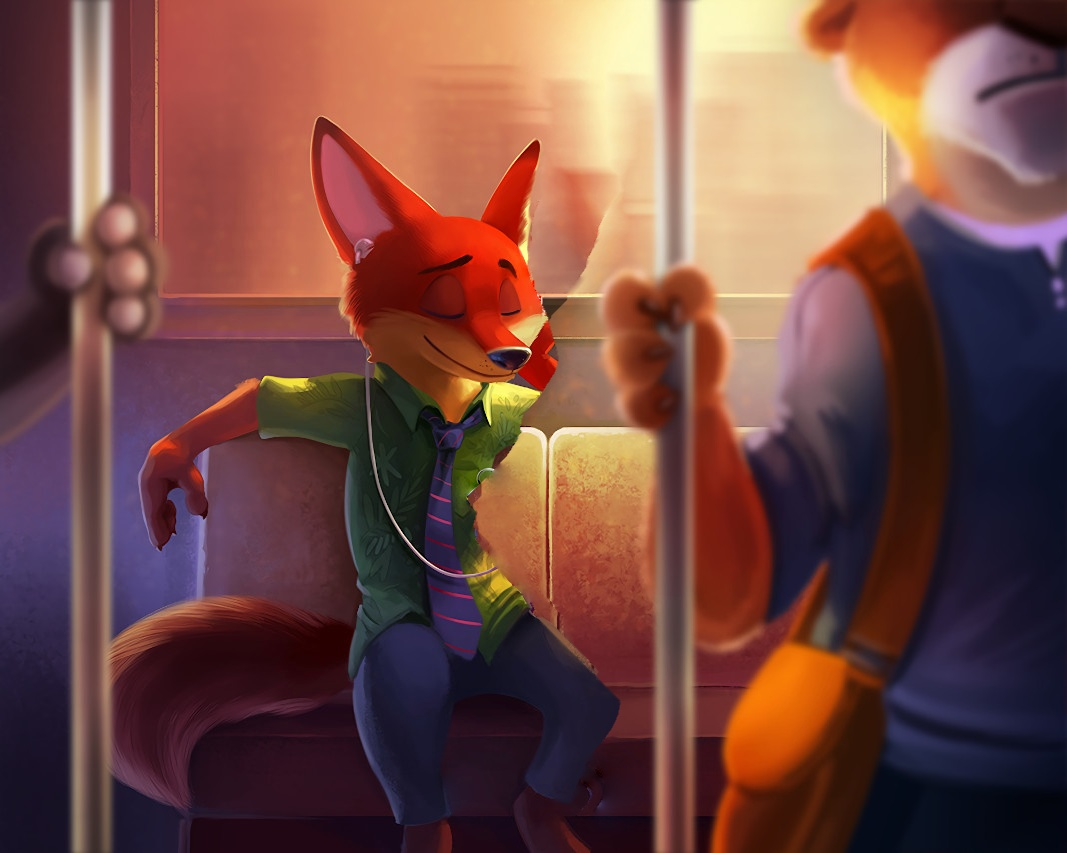
\includegraphics[height=4cm,trim=350 200 350 400,clip]{demo/output/zootopia_poisson.jpg}
    }
    \caption{使用Poisson Solver进行目标移除的效果}
    \label{fig:poisson_removal}
\end{figure}\par
下面是\cite{avidan2007seam}中提供的样例,直接缩小的方法相比原文没有明显的颜色不连续现象,此时使用Poisson Solver得到的结果没有明显优势。
\begin{figure}[H]
    \centering
    \subfigure[直接缩小]{
        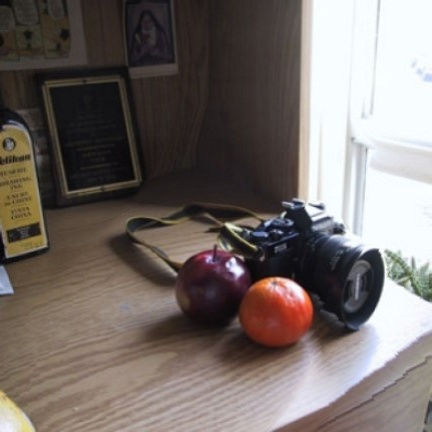
\includegraphics[height=6cm]{demo/output/poisson_disabled.jpg}
    }
    \subfigure[使用Poisson Solver]{
        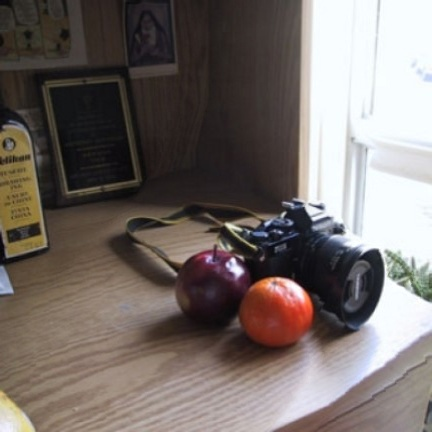
\includegraphics[height=6cm]{demo/output/poisson_enabled.jpg}
    }\\
    \subfigure[直接缩小(局部)]{
        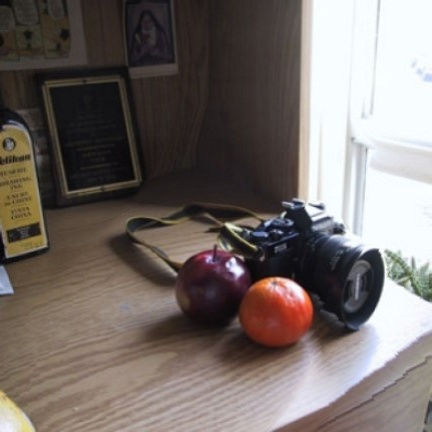
\includegraphics[trim=0 120 300 100,clip,height=6cm]{demo/output/poisson_disabled.jpg}
    }
    \subfigure[使用Poisson Solver(局部)]{
        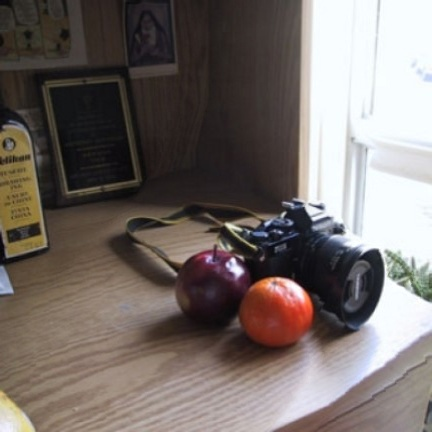
\includegraphics[trim=0 120 300 100,clip,height=6cm]{demo/output/poisson_enabled.jpg}
    }
    \caption{使用Poisson Solver进行图像缩小的效果}
    \label{fig:poisson_resize}
\end{figure}\par
\bibliographystyle{plain}
\bibliography{refs}
\end{document}
